\section{Misalignment Studies} \label{sec:misalign}

To protect both the active area of the SiPMs and the scintillator surface at the upstream end of the straight section, the coupling distance between the two was required to be larger than zero.  Similarly, the scintillator paddles were also shimmed radially such that the top edge of the scintillator was level with the top edge of the active area of the SiPM thereby maximizing light collection.  It was therefore necessary to study the effects of SiPM/scintillator misalignments on light collection and time resolution.

The SiPM sits atop a Newport MT-XYZ (MT) compact dovetail XYZ linear translation stage with three fine adjustment screws with 80 threads per inch as seen in Fig. \ref{fig:sipm_trans_stage}.  
\begin{figure}[!htb]
	\centering
	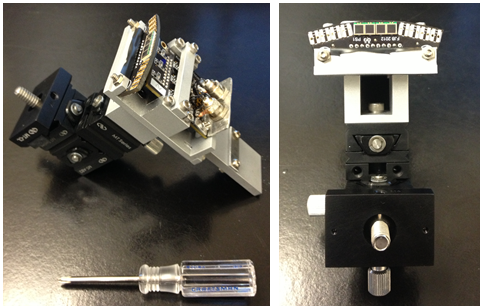
\includegraphics[width=1.0\columnwidth]{misalignment/figs/sipm_trans_stage}
	\caption{The SiPM case is the aluminum matt finished metal.  The translation stage is black. Left: isometric view of SiPM case and MT-XYZ translation stage.  Right:  front view (looking upstream).}
	\label{fig:sipm_trans_stage}
\end{figure}
Each translation knob for the three axes of translation provides a translation of $318\ \mathrm{\mu m}$ per rotation.  It is useful to note that for each location of the SiPM, relative to the scintillator, the source and trigger PMT were located at $z = 24.467$ cm and 10,000 event triggers were collected.  %Furthermore, paddle 5 from the third batch of machined scintillator paddles from McNeal was used for these studies. 

\subsection{Vertical Alignment of SiPM \& Scintillator}
\label{sec:vertical alignment of SiPM and Scintillator}

To study the effects of the various horizontal (translations along the $z-axis$) coupling distances, the relative position of the active area of the SiPM and the top edge of the scintillator paddle was required to be known.  Vertical alignment is the most critical since the 3 mm thickness of the scintillator matches the 3 mm height of the active area of the SiPM.  To test the 50 machined scintillators in a reproducible manner, the vertical alignment of the SiPM and scintillator must be replicated in a robust manner.

Utilizing an Edmund Optics CMOS camera, and a ruler (seen in Fig. \ref{fig:sipm_va_optics}) the vertical alignment of the top edges of the SiPM and scintillators could be measured within 0.025 mm accuracy relative to the ST2 PCB Board.
\begin{figure}[!htb]
	\centering
	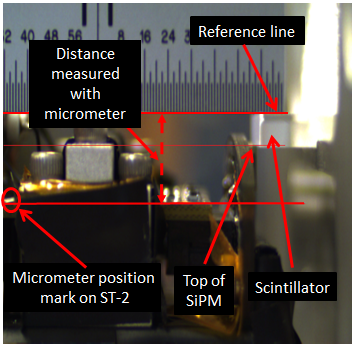
\includegraphics[width=1.0\columnwidth]{misalignment/figs/sipm_va_optics}
	\caption{Vertical alignment optics set-up.  The reference line corresponds to the top surface of the scintillator, while the micrometer position on the ST2 is clearly marked so that the absolute difference could be measured both optically and manually with a micrometer.}
	\label{fig:sipm_va_optics}
\end{figure}
The $3 \times 3\ \mathrm{mm^{2}}$ SiPMs, which are mounted to the ST1, are housed in a ceramic case mounted on the ST1 PCB.  Therefore, there exists some area between the top of the SiPM ceramic case and the active area of the SiPM which must be taken into account.  The distance is also measured both optically and manually relative to the ST2 PCB.

Figure \ref{fig:sipm_va_optics_schematic} illustrates a labelled schematic similar to what was seen in Fig. \ref{fig:sipm_va_optics} and depicts the variables measured and monitored so as to quantify the vertical alignment.
\begin{figure}[!htb]
	\centering
	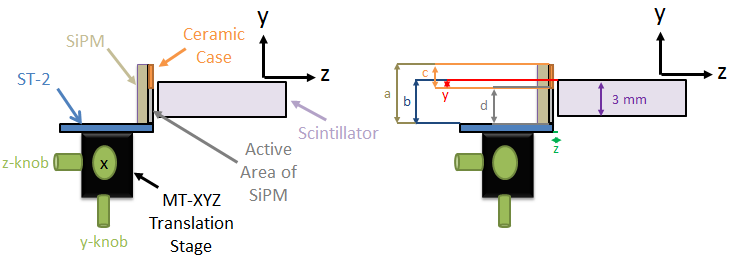
\includegraphics[width=1.0\columnwidth]{misalignment/figs/sipm_va_optics_schematic}
	\caption{Vertical alignment optics schematic.  Left: labelled cartoon of SiPM \& scintillator vertical alignment.  Right: variables used to quantify vertical alignment.  The scintillator is intentionally misaligned in this cartoon so that the misalignment parameter y is visible.}
	\label{fig:sipm_va_optics_schematic}
\end{figure}
Of all the variables in Fig. \ref{fig:sipm_va_optics_schematic}, $y$ is of the utmost importance since it is the distance between the top edge of the scintillator paddle and the active area of the SiPM and is the quantization of the vertical misalignment.  That is to say the at $y = 0$ the SiPM and scintillator are aligned vertically.  Both the distance between the top of the SiPM and ST2 PCB ($a$), and the distance between the top of the SiPM and the active area of the SiPM ($c$), are measured optically and define the distance between the top edge of the active area of the SiPM and the ST2 PCB ($d$) \textit{via} $d = a - c$, which are all constants. It is necessary to note that the coupling distance between the active area of the SiPM and scintillator ($z$) was done by eye and then measured optically until a desirable coupling distance was found.  The values of the aforementioned variables are summarized in Table \ref{tab:va_vars}.
\begin{table}[!htb]
	\centering
	\begin{tabular}{|c|c|}
		\hline \textbf{Variable} & \textbf{Value (mm)} \\ 
		\hline a & 5.22 \\ 
		\hline c & 0.91 \\ 
		\hline d & 4.32 \\ 
		\hline z & 0.25 \\ 
		\hline 
	\end{tabular} 
	\caption[Vertical alignment variables]{Vertical alignment variables.  All variables were measured five times and the numbers reported are averages of those values.}
	\label{tab:va_vars}
\end{table}
The variable $b$ defines the distance between the top edge of the scintillator and the ST2 PCB and is measured both optically and manually.  This distance, coupled with the constant $d$, provides the measured quantity $y$ through the difference $y = b - d$.

The coordinate system used to quantify the vertical misalignment studies is illustrated in Fig. \ref{fig:sipm_va_schematic}.
\begin{figure}[!htb]
	\centering
	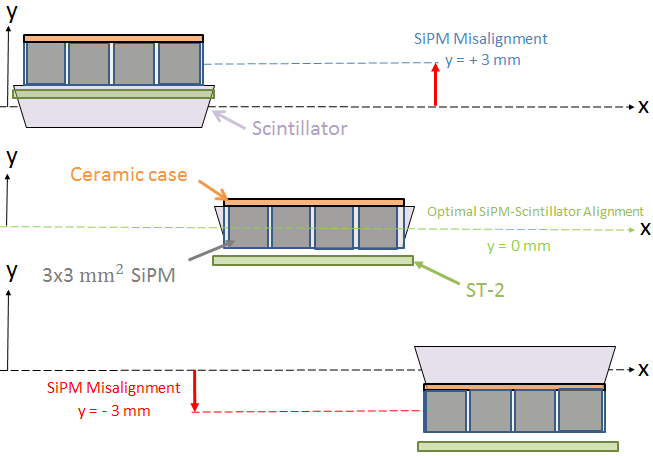
\includegraphics[width=1.0\columnwidth]{misalignment/figs/sipm_va_schematic}
	\caption{Vertical alignment schematic.  The scintillator is fixed while the SiPM effectively scans across the face of the scintillator along the y-axis.}
	\label{fig:sipm_va_schematic}
\end{figure}
The scintillator remained fixed, while the SiPM was lowered, relative to the scintillator, to the minimum location governed by the range of the MT translation stage at approximately $y = -4$ mm.  Coarse measurements were then taken at half turns $(159\ \mathrm{\mu m})$ intervals until the maximum height of the MT translation stage was reached which was approximately $y = +4\ \mathrm{mm}$.  The results of these measurements can be seen in Fig. \ref{fig:sipm_va_coarse}.
\begin{figure}[!htb]
	\centering
	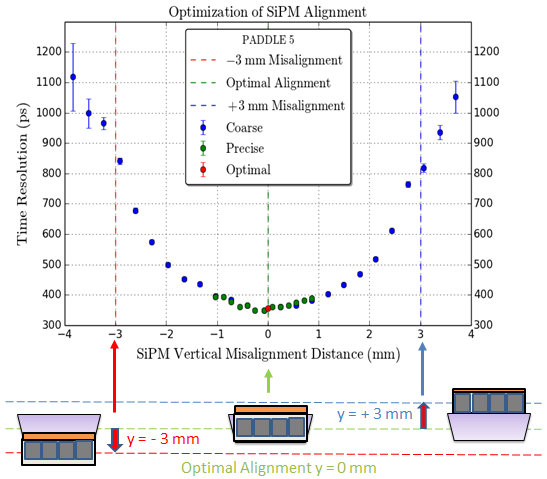
\includegraphics[width=1.0\columnwidth]{misalignment/figs/sipm_va_coarse}
	\caption{Coarse vertical misalignment results.  The minimum time resolution obtained was approximately 350 ps which was expected.  Once the SiPM exceeded $y = \pm 3\ mm$ there is no active area of the SiPM coupled to the face of the scintillator.}
	\label{fig:sipm_va_coarse}
\end{figure}
Once the coarse measurements concluded, the SiPM was lowered to $y \approx -1$ mm and then the translation stage was moved in quarter turn $(79.5\ \mathrm{\mu m})$ intervals until $y \approx +1\ \mathrm{mm}$ was reached.  The results of both the coarse and fine measurements are seen in Fig. \ref{fig:sipm_va_fine}.
\begin{figure}[!htb]
	\centering
	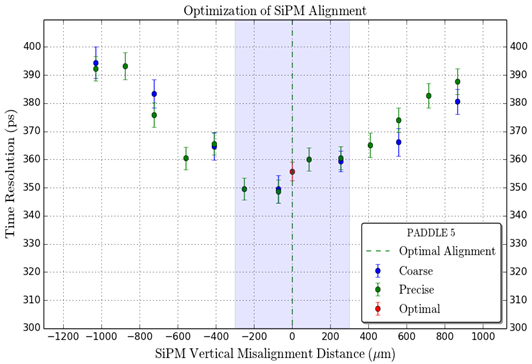
\includegraphics[width=1.0\columnwidth]{misalignment/figs/sipm_va_fine}
	\caption{Fine vertical misalignment results.  Note that the coarse and fine measurements were overlapped so the reproducibility of the measurements were depicted.}
	\label{fig:sipm_va_fine}
\end{figure}
It is useful to note that at every location of the SiPM the distance traversed was verified by a manual measurement made with a micrometer ($1\ mil$ precision).

From the vertical misalignment studies it is clear that there is no significant variation of time resolution within a $\pm 300\ \mathrm{\mu m}$ range of the ideal alignment.  These results were also simulated in a manner similar to what was discussed in section \ref{sec:simulating the machined scintillator geometery} and the results are seen in Fig. \ref{fig:vertical_sim}.
\begin{figure}[!htb]
	\centering
	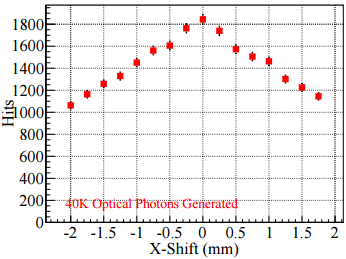
\includegraphics[width=1.0\columnwidth]{misalignment/figs/vertical_sim}
	\caption{Vertical alignment simulation studies \cite{puneet_sim_talk}.  It is important to note the x-axis corresponds to the y-axis as discussed with the experimental measurements.}
	\label{fig:vertical_sim}
\end{figure}
The Geant4 simulations indicate that the acceptable range of vertical misalignment is approximately $\pm 250\ \mathrm{\mu m}$ \cite{puneet_sim_talk} which is consistent with what was measured on the bench at FIU.

\subsection{Coupling Distance of SiPM \& Scintillator}

With the vertical alignment between the scintillator and SiPM optimized, the effects of varying the coupling distance was studied.  Using an identical set-up as was described in section \ref{sec:vertical alignment of SiPM and Scintillator} the coupling distance, and resulting time resolutions, was measured at various locations with three distances shown in Fig. \ref{fig:sipm_coupling_optics}.  
\begin{figure}[!htb]
	\centering
	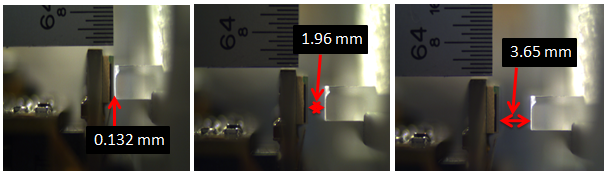
\includegraphics[width=1.0\columnwidth]{misalignment/figs/sipm_coupling_optics}
	\caption{Coupling distance optics. Various coupling distances as measured with the CMOS camera.  The high degree of precision is clearly visible.}
	\label{fig:sipm_coupling_optics}
\end{figure}
While the coupling distance was varied, the vertical alignment was kept constant at the optimal location determined from the studies outlined in section \ref{sec:vertical alignment of SiPM and Scintillator} and was monitored both optically and manually.

With the optimal vertical alignment having been verified, the SiPM was moved \textit{via} the MT translation stage along the $z-axis$ such that the active area of the SiPM was flush against the face of the machined scintillator paddle at $z = 0\ \mathrm{mm}$.  In the coupling region $z < 1\ \mathrm{mm}$ the SiPM was receded from the face of the SiPM in 1/4 turn ($79.5\ \mathrm{\mu m}$) intervals.  For $\mathrm{1\ mm < z < 2\ mm}$, the SiPM was receded from the face of the SiPM in 1/2 turn ($159\ \mathrm{\mu m}$) intervals, and for $\mathrm{2\ mm < z < 4\ mm}$ data were collected in 1 turn ($\mathrm{318\ \mu m}$) intervals and is illustrated in Fig. \ref{fig:sipm_coupling_coarse}.
\begin{figure}[!htb]
	\centering
	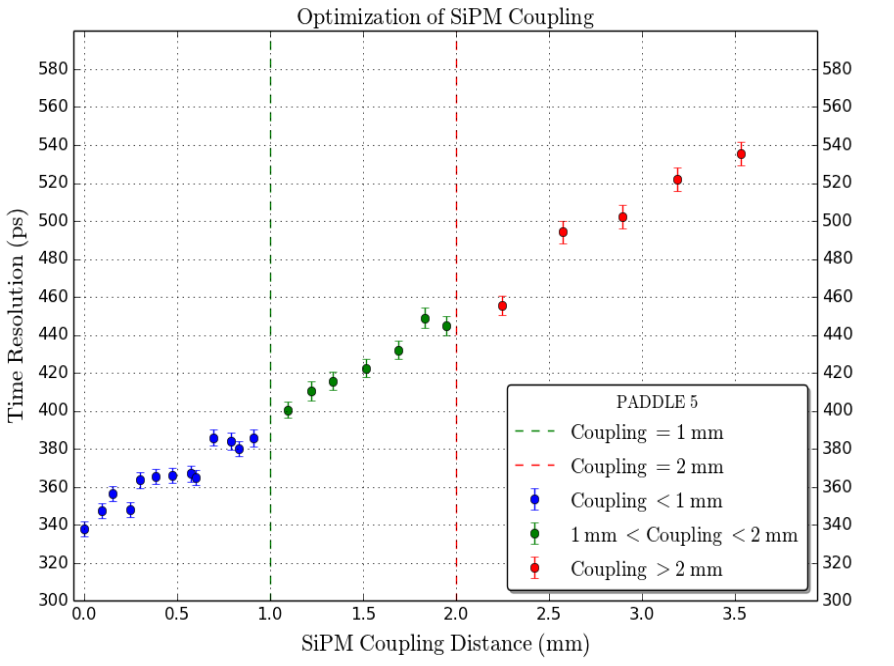
\includegraphics[width=1.0\columnwidth]{misalignment/figs/sipm_coupling_coarse}
	\caption{Coarse coupling distance studies.  It is useful to note that at a coupling distance of $\mathrm{251\ \mu m}$ the time resolution was identical to what was measured in Fig. \ref{fig:sipm_va_fine} while conducting the vertical alignment studies.}
	\label{fig:sipm_coupling_coarse}
\end{figure}

Figure \ref{fig:sipm_coupling_fine} zooms in on the ($\mathrm{z < 1\ mm}$) region of the coupling distance studies shown in Fig. \ref{fig:sipm_coupling_coarse}.
\begin{figure}[!htb]
	\centering
	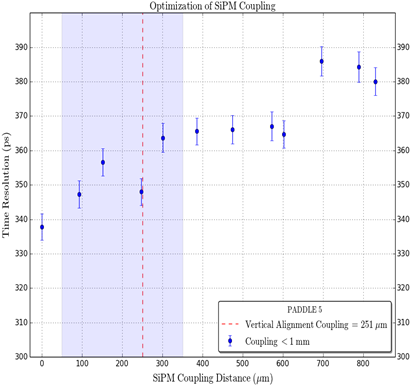
\includegraphics[width=1.0\columnwidth]{misalignment/figs/sipm_coupling_fine}
	\caption{Fine coupling distance studies.  The blue shaded region ($50\ \mu m < z < 350\ \mu m$) indicates the optimal coupling range.}
	\label{fig:sipm_coupling_fine}
\end{figure}
It is clear from the data the optimal coupling range was $\mathrm{50\ \mu m < z < 350\ \mu m}$ and there was no significant reduction in time resolution performance over a $\mathrm{0\ \mu m < z < 600\ \mu m}$ range.  Similarly, the simulation results also indicate that there is no significant reduction in light collection in the $\mathrm{0\ \mu m < z < 600\ \mu m}$ range \cite{puneet_sim_talk}.
\begin{figure}[!htb]
	\centering
	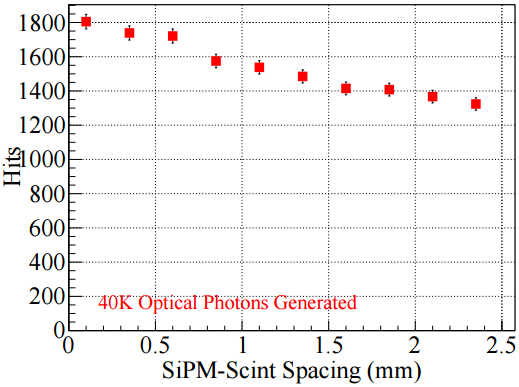
\includegraphics[width=1.0\columnwidth]{misalignment/figs/spacing_sim}
	\caption{Coupling distance simulations. Simulations indicated that the optimal coupling distance is in the $50\ \mu m < z < 350\ \mu m$ range.}
	\label{fig:spacing_sim}
\end{figure}


